\textbf{Questions/Remarks}
\begin{itemize}
    \item $B_a\Phi(\sigma)$ = constant when using only one modeshape to  approximate strains, right? Because all shape function values will return 1, no matter what $\sigma$ is.
    \item Mass of the actual robot 
    \item Slice thickness even smaller, maybe means analytically solve for g'
\end{itemize}




\section{Stiffness Determination}


As far as I am concerned the stiffnesses have now been correctly determined. E.g. the kinematic model is fit to the actual data, so no scaling was used. For the elongation (which is unit less) this does not give any/much differences. However, the curvature stiffness changed a great deal.  The figures below show the  new fits and the parameters of the hyper-elastic stiffness model are presented in the Table.


\begin{figure}[H]
    \centering
\begin{minipage}{0.5\textwidth}
        \centering
        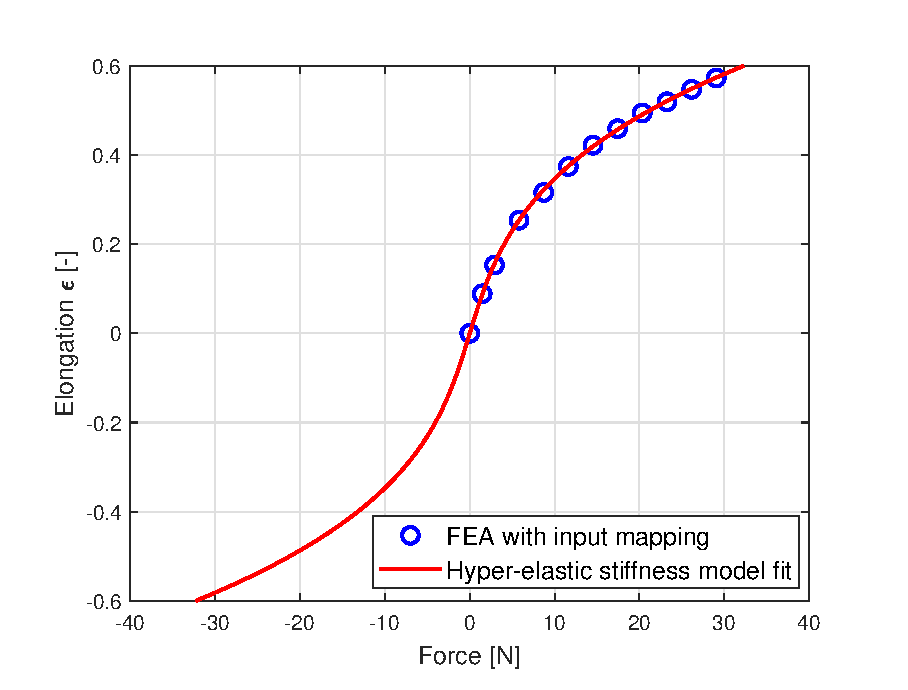
\includegraphics[width=\textwidth]{Figures/Chapter3/mappedforcevselongation.eps}
        \caption{Fitted stiffness model for elongation.}
    \end{minipage}\hfill
    \begin{minipage}{0.5\textwidth}
        \centering
        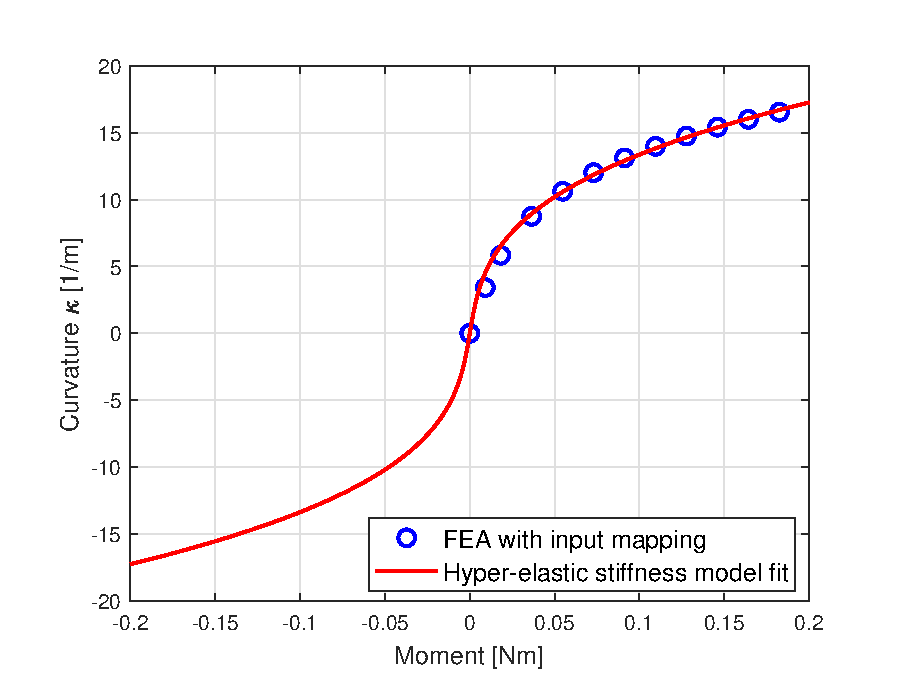
\includegraphics[width=\textwidth]{Figures/Chapter3/mappedmomentvscurvature.eps} 
        \caption{Fitted stiffness model for curvature.}
    \end{minipage}
\end{figure}

\begin{table}[H]
    \centering
        \caption{Parameters for hyper-stiffness model.}
\begin{tabular}{|c|c|c|c|} \hline
            &  $i = $ 1      &    $i = $    2   &  $i = $ 3  \\ \hline
   $\alpha_i \hspace{2pt}[N]$    &    1.3936e+3    & 1.3776e+3    & 2.7865e-1 \\ \hline
   $\beta_i \hspace{2pt}  [Nm^2] $     &  3.0322 & 3.0309    &  3.3755e-3\\ \hline
\end{tabular}
\end{table}


\section{Determination of non-linear mass matrix}

I will briefly discuss how this is currently determined. I think the approach you told me was implemented correctly. However, I doubt there are still some bugs. Luckily the oscillatory behaviour looks like expected. The thing I worry about are the large elongations that are observed. Ofcourse the observed behaviour depends largely on the chosen parameters. Such as mass and damping. The oscillation timescale is reasonable I think.  I have not been able to work everything out very well. Therefore it might be best to show the equations that I used and some code snippets to get an idea on the implementation. Lastly I will show a simulation.

Assume the total kinetic energy of the system is equal to 

\begin{equation}
    T = \frac{1}{2} \int_0^L VM(\sigma)V d\sigma
\end{equation}

where $M = \text{diag}([m_x,m_y,m_z,I_{xx},I_{yy},I_{zz}])$, since it is assumed that $m$ is a point mass it holds that $m_x=m_y=m_z$. And assume we can write V as,

\begin{equation}
    V = J\dot{q},
\end{equation}

Where $J$ can be formulated as,
\begin{equation}
    J = Ad_g^{-1}(\sigma) \int_0^L Ad_g(\sigma) B_a\Phi(\sigma)d\sigma
\end{equation}

Substitution gives,

\begin{equation}
    T = \frac{1}{2}\int_0^L (J(\sigma)\dot{q})^\top M(\sigma) J(\sigma)\dot{q} d\sigma
\end{equation}

This allows to define a mass matrix dependent on modal coordinates $q$ as,

\begin{equation}
    M(q) = J(\sigma)^\top M(\sigma) J(\sigma) 
\end{equation}

The mass matrix is determined using the script below. I will explain it in more depth tomorrow.
\newpage

\begin{lstlisting}

%% At each time instant the forward kinematic sript is ran for kappa and epsilon hence q = [k,e]
Q0 = rot2quat(eye(3));
r0 = zeros(3,1);
g0 = [Q0;r0];


[l, g] = ode45(@(l,g) forwardKinematics(l,g,q,Ba,shape,Nmode,L),[0 L],g0); % solve forward kinematics

%% Interpret data
R = g(:,1:4);       % robot's rotation expressed in quaternions
r = g(:,5:7);

G = 0;
Mq = 0;
    
    for ii = 2:length(l) % numerically integrate [0,L] G = int(Adg*Ba*Phi(sigma)dsigma) [0,L]
        
        dsigma = l(ii)-l(ii-1);     % slice thickness
        sigma = l(ii);              % sigma in [0,L]
        Baphi_s = shapeValue(shape,Nmode,sigma,Ba,L);    % Determine Ba*Phi_s for each sigma
        Adg = adjointG(R(ii,:),r(ii,:));                 % Calculate Adg for each sigma   
        G = G + Adg*Baphi_s*dsigma;
        
    end
         
   for jj = 2:length(l)
        dsigma = l(jj)-l(jj-1); % slice  thickness 
        AdgInv = adjointGInv(R(jj,:),r(jj,:)); 
        [m_sigma,Jxx,Jyy,Jzz] = inertiaRectangle(m,L,w,d,dsigma); 
        M = diag([Jxx,Jyy,Jzz,m_sigma,m_sigma,m_sigma]);  % curvature and elongation are swapped here Ba is defined as [K;E]
        J = AdgInv*G;      % J(sigma) = Adg^-1(\sigma) G
        Mq = Mq + J'*M*J;   % sum over all M
  
    end

   Mq = rot90(Mq,2)';      % flip diagonally, here q = [k,e] in SS [e,k]
\end{lstlisting}

\subsection{Simulation results}

The image below shows the step response of a system with initital conditions $x_0 = [\epsilon \hspace{4pt} \kappa \hspace{4pt} \dot{\epsilon} \hspace{4pt} \dot{\kappa}] =  [0.2 \hspace{4pt} 0 \hspace{4pt} 0 \hspace{4pt} 0]$. Damping matrix $D = \text{diag}([0.03,0.000012])$, mass of the actuator $m = 0.030\hspace{4pt}  [kg]$ and input $p_i = 0 \hspace{4pt} \text{for} \hspace{4pt} t  < 0.05 \hspace{4pt}  \text{else} \hspace{4pt} 40 \hspace{4pt}  [kPa]$ .

\begin{figure}[H]
    \centering
    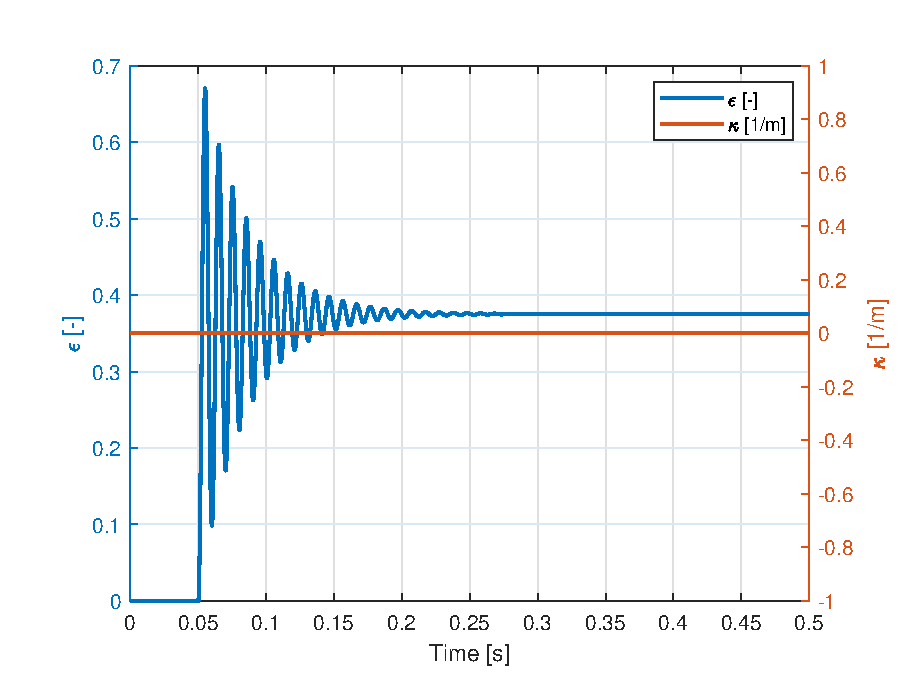
\includegraphics{Figures/ProgresFigures/sim1.eps}
    \caption{Simulation}
    \label{fig:my_label}
\end{figure}

As you can see the oscillation time is 0.2 seconds for a step response causing an elongation. It is however odd that this results in an elongation of 0.68, implying that the actuator will increase its length 1.68x. Several things could cause this behaviour. I will look at this further tomorrow.